\documentclass[]{article}
\usepackage[utf8]{inputenc}
\usepackage[ngerman]{babel}
\usepackage[T1]{fontenc}
\usepackage{%
	ngerman,
	ae,
	times,  %% hier kann man die Schriftart einstellen
	graphicx,
	url,
	scrlayer-scrpage,
	lastpage,
	mathtools,
	geometry,
	multicol,
	cancel,
	xcolor,
	nicematrix,
	xfrac,
	tikz,
	pgfplots,
	amsmath,
	colortbl,
	centernot,
	dsfont,
	textgreek,
	icomma,
	pdfpages}
\usepackage[thinlines]{easybmat}
\usetikzlibrary{datavisualization}
\usetikzlibrary{datavisualization.formats.functions}
\usetikzlibrary{intersections}
\pgfplotsset{compat=1.17}
\newcommand{\del}[1]{\cancel{~#1~}}
\NiceMatrixOptions{ last-col,code-for-last-col = \color{blue}\scriptstyle,light-syntax}
\newlength\dlf
\newcommand\alignedhighlight[3]{
  % #1 = color
  % #2 = before alignment
  % #3 = after alignment
  &
  \begingroup
  \settowidth\dlf{$\displaystyle #2$}
  \addtolength\dlf{\fboxsep+\fboxrule}
  \hspace{-\dlf}
  \fcolorbox{#1}{#1}{$\displaystyle #2 #3$}
  \endgroup
}
\newcommand{\reference}[1]{ \text{\small{\textcolor{blue}{(#1)}}} }

\newcommand{\topic}{Grundlagen Technische Informatik}
\newcommand{\subtopic}{Versuch 1}
\newcommand{\authors}{Kleingruppe A2}

%Head and Footnotes
\setlength{\headheight}{2.1\baselineskip} %baselineskip = minimum distance bbetween the bottom of one line to another.
\geometry{bottom = 3cm}
\setlength{\headsep}{\baselineskip}
\ihead[\topic\hrule]{\topic\hrule}
\chead[\subtopic\\~]{\subtopic\\~}
\ohead[\authors\\~]{\authors\\~}
\ifoot[~]{~}
\cfoot[~]{~}
\ofoot[Seite \thepage~von \pageref{LastPage}]{Seite \thepage~von \pageref{LastPage}}

%Paragraph spacings
\setlength{\parindent}{0em} %em = with of an 'M'
\setlength{\parskip}{1ex} %ex = height of an 'x'


\newcommand{\V}{\lor}
\newcommand{\A}{\land}
\newcommand{\T}[1]{\overline{#1}}
\newcommand{\eq}{\Leftrightarrow}
\newcommand{\rarr}{\Rightarrow}
\newcommand{\red}[1]{\textcolor{red}{#1}}

\newcommand{\unit}[1]{\text{#1}}
\newcommand{\fracunit}[2]{\frac{\unit{#1}}{\unit{#2}}}
\newcommand{\textsq}[1]{\ensuremath{\text{#1}^2}}
\newcommand{\textpow}[2]{\ensuremath{\text{#1}^{#2}}}
\newcommand{\tdot}{\ensuremath{\cdot}}


\begin{document}
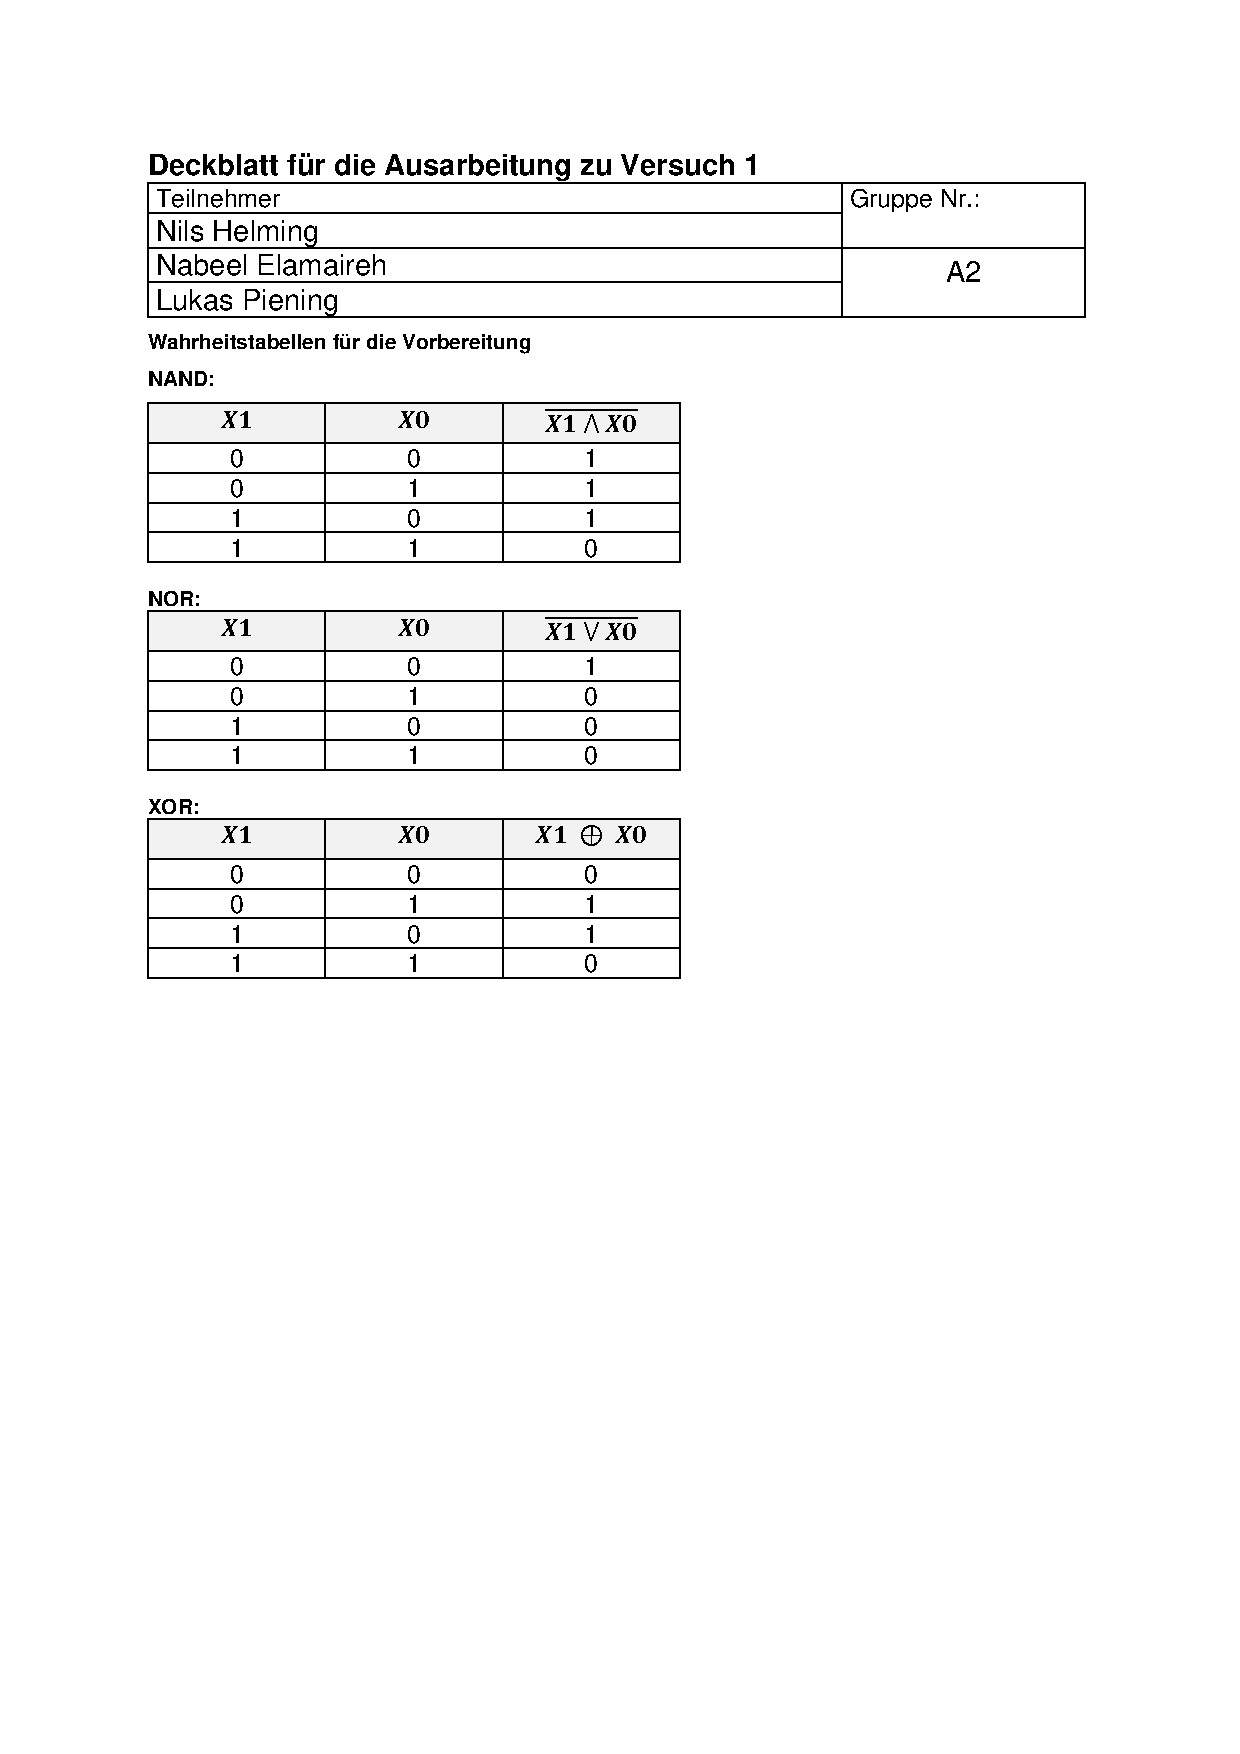
\includepdf[pages=-]{Versuch1H_Deckblatt.pdf}
\section*{Vorbereitung}
	\begin{align*}
		\text{Disjunktive Normalform von XOR:}&\\
		X_1 \oplus X_2 &= m_1 \V m_2 = (\T{X_1} \A X_2) \V (X_1 \A \T{X_2})\\
		\text{Umformung in NAND und Inverter:}&\text{ (2. De Morgansches Gesetz)}\\
		X_1 \oplus X_2 &= (\T{X_1} \A X_2) \V (X_1 \A \T{X_2})\\
		&= \T{\T{\T{X_1} \A X_2} \A \T{X_1 \A \T{X_2}}}\\
	\end{align*}
\section*{Aufgabe 1: Simulation von Logik-Gattern mit Logisim-Evolution}
\subsection*{1a)}
	\begin{center}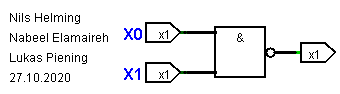
\includegraphics[scale=0.7]{Bilder/1_a.png}\end{center}
\subsection*{1b)}
	\begin{center}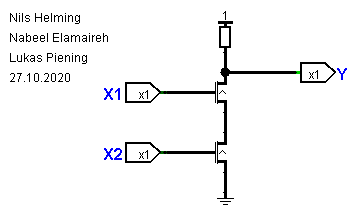
\includegraphics[scale=0.7]{Bilder/1_b.png}\end{center}
\subsection*{1c)}
	\begin{center}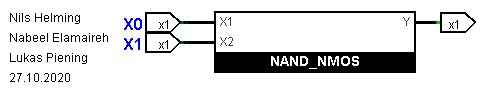
\includegraphics[scale=0.7]{Bilder/1_c.png}\end{center}
\subsection*{1d)}
	\begin{center}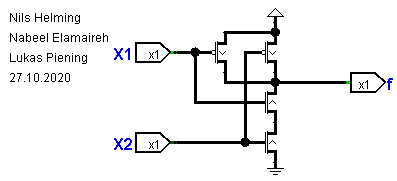
\includegraphics[scale=0.7]{Bilder/1_d.png}\end{center}
\subsection*{1e)}
	Disjunktive Normalform von NOR:
	$f(X_1, X_2) = \T{X_1 \V X_2} = m_1 = \T{X_1} \A \T{X_2}$


	$h(X_1, X_2) = f(X_1, X_2) = \T{X_1} \A \T{X_2}$\\ Hier sind keine Änderungen nötig, da alle Eingänge schon negiert sind. Das $\A$ wird in dem Schaltungsgatter in einer Reihenschaltung umgesetzt.


	$g(X_1, X_2) = \T{f(X_1, X_2)} = \T{\T{X_1} \A \T{X_2}} = X_1 \V X_2$\\
	Das $\V$ wird in dem Schaltungsgatter in einer Parallelschaltung umgesetzt.
	\begin{center}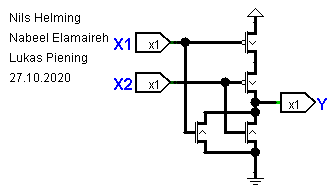
\includegraphics[scale=0.7]{Bilder/1_e.png}\end{center}
\subsection*{1f)}
	\begin{center}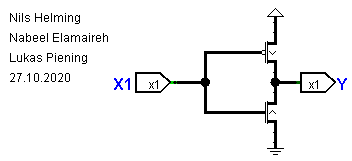
\includegraphics[scale=0.7]{Bilder/1_f.png}\end{center}
\subsection*{1g)}
	\begin{center}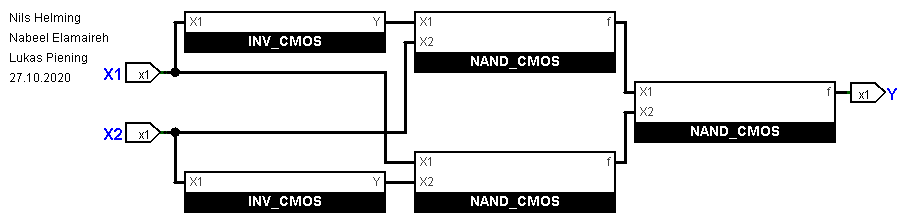
\includegraphics[scale=0.45]{Bilder/1_g.png}\end{center}


\section*{Aufgabe 2: Normalformen einfacher Schaltungen}
	\begin{multicols}{2}
		Minterme:\\
		$m_0 = \T{X_2} \A \T{X_1} \A \T{X_0}$\\
		$m_1 = \T{X_2} \A \T{X_1} \A 	X_0$\\
		$m_2 = \T{X_2} \A     X_1 \A \T{X_0}$\\
		$m_3 = \T{X_2} \A     X_1 \A    X_0$\\
		$m_4 =     X_2 \A \T{X_1} \A \T{X_0}$\\
		$m_5 =     X_2 \A \T{X_1} \A    X_0$\\
		$m_6 =     X_2 \A     X_1 \A \T{X_0}$\\
		$m_7 =     X_2 \A     X_1 \A    X_0$\\


		Maxterme:\\
		$M_0 =     X_2 \V  	  X_1 \V    X_0 $\\
		$M_1 =     X_2 \V     X_1 \V \T{X_0}$\\
		$M_2 =     X_2 \V \T{X_1} \V 	X_0 $\\
		$M_3 =     X_2 \V \T{X_1} \V \T{X_0}$\\
		$M_4 = \T{X_2} \V     X_1 \V    X_0 $\\
		$M_5 = \T{X_2} \V     X_1 \V \T{X_0}$\\
		$M_6 = \T{X_2} \V \T{X_1} \V    X_0 $\\
		$M_7 = \T{X_2} \V \T{X_1} \V \T{X_0}$\\
	\end{multicols}
\subsection*{$Y_1$:}
	Konjunktive Normalform von $Y_1$ ist die Konjunktion (UND) der Maxterme, dessen Zeilen in der Wahrheitstabelle $0$ darstellen\\

	\begin{align*}
	Y_1 = M_1 \A M_5 \A M_7 =
		(X_2 \V     X_1 \V \T{X_0}) \A    %M1
		(    \T{X_2} \V     X_1 \V \T{X_0}) \A  %M5
		(   \T{X_2} \V \T{X_1} \V \T{X_0})\\    %M7
	\end{align*}

	Disjunktive Normalform von $Y_1$ ist die Disjunktion (ODER) der Minterme, dessen Zeilen in der Wahrheitstabelle $1$ darstellen\\

	\begin{align*}
		Y_1 &= m_0 \V m_2 \V m_3 \V m_4 \V m_6\\
		&=
		(\T{X_2} \A \T{X_1} \A \T{X_0}) \V
		(\T{X_2} \A     X_1 \A \T{X_0}) \V
		(\T{X_2} \A     X_1 \A    X_0) \V
		(    X_2 \A \T{X_1} \A \T{X_0}) \V
		(    X_2 \A     X_1 \A \T{X_0})
	\end{align*}


\end{document}